\documentclass[12pt, a4paper, twoside]{article}
\usepackage[utf8]{inputenc}

\title{Update of the register size used in the NeXtRad Synchronization Controller}
\author{Dominic Manthoko}
\date{\today}

%package needed in order to use images
\usepackage{graphicx}
\graphicspath{{images/}{images/tcu/}{images/tcu_external_clock}}

\begin{document}

%\begin{titlepage}
\maketitle
%\end{titlepage}

%Deals with the text being too long to fill one line
%E.g Background of the NeXtRad...
\sloppy


\section{Introduction}

\subsection{Subject and Motivation of Report}
The author was requested to make modifications to the NeXtRad Synchronization Controller developed by Johann Burger. In particular, the register size of the Synchronization Controller needed to be increased from 16 bits to 32 bits. 

\subsection{Background of the NeXtRad Synchronization Controller}


\subsection{Methodology}

\section{Modifications of the Synchronization Controller}


\section{Experimental setup}

	\begin{figure}[h]
		\centering
		\includegraphics[width=13cm]{experimental_setup}
		\caption{Picture of the equipment used to test the 32 bit version of the synchronization controller}
		\label{fig:exp_setup}
	\end{figure}
	
The experimental setup used to test the modified controller can be seen in figure \ref{fig:exp_setup}. A signal generator operating at 100MHz with an amplitude of +550mV was used as the input clock. This clock signal was passed through a diode then fed into the rhino. An oscilloscope was used to measure the Main bang offset and Digitisation signals coming out of the rhino. 
	
	
\section{Results of the Experiment}

\subsection{Using the Rhino Board Internal 100MHz clock}

Testing of the modified synchronization controller began with using the internal clock of the Rhino board. Using the internal clock, 1kHz, 2kHz, 3kHz and 4kHz signals were produced. 

	\begin{figure}[h]
		\centering
		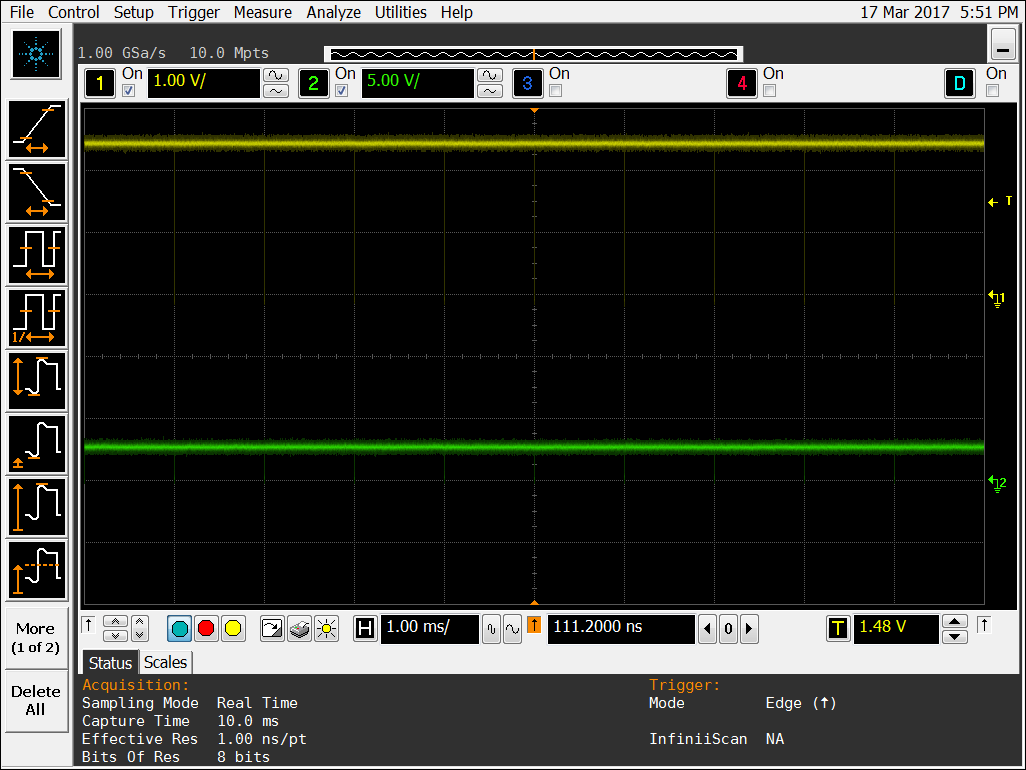
\includegraphics[width=13cm]{1khz_mb_offset_500_ns}
		\caption{1khz signal produced using the internal clock of the rhino}
		\label{fig:1khz_in_500_offset}
	\end{figure}
	
Figure \ref{fig:1khz_in_500_offset} shows the output of the main bang and the digitisation signals measured from the Rhino board. A time division of 1.0 ms was used to display the output.

\subsection{Using an External 100MHz Clock Signal}


\section{Conclusions}

\section{Recommendations}

\end{document}